\documentclass[a4paper,12pt]{article}
\usepackage[margin=2.5cm]{geometry}
\usepackage{graphicx}
\usepackage{float}
\usepackage{subcaption}

\begin{document}

\vspace*{0pt}
\begin{center}
\Large Project 2 - Fractal Plots
\end{center}

For the following plots I used the polynomial
\[
P(z) = (1+i) + (2+2i)z + (3+3i)z^2 + (4+4i)z^3 + (5+5i)z^4 + (6+6i)z^5
\]
where the origin is at $-2+i$ and the square has a width of $2$.

\begin{figure}[H]
    \centering
    % First subfigure
    \begin{subfigure}[b]{0.48\linewidth} % about half the width
        \centering
        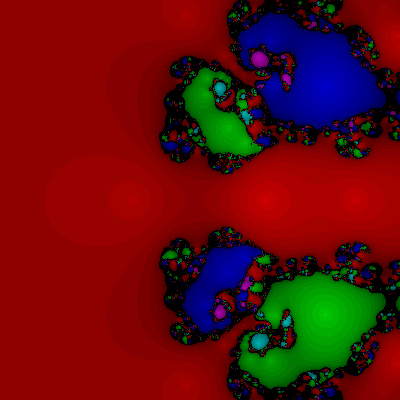
\includegraphics[width=\linewidth,keepaspectratio]{fractal-dark.png}
        \caption{Fractal dark}
        \label{fig:fractal1}
    \end{subfigure}
    \hfill % adds space between images
    % Second subfigure
    \begin{subfigure}[b]{0.48\linewidth}
        \centering
        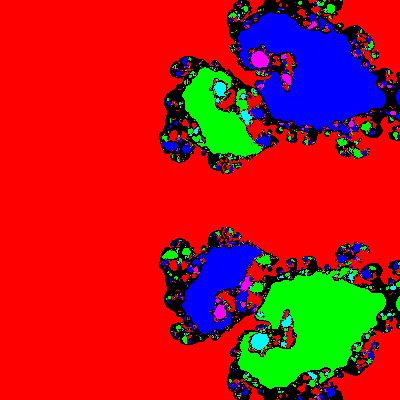
\includegraphics[width=\linewidth,keepaspectratio]{fractal-light.png}
        \caption{Fractal light}
        \label{fig:fractal2}
    \end{subfigure}
    \caption{Fractal plots side by side}
    \label{fig:fractal-both}
\end{figure}

\end{document}
